\documentclass[a4paper, 11pt, final, garamond]{book}
\usepackage{cours-preambule}

\raggedbottom

\makeatletter
\renewcommand{\@chapapp}{Programme de kh\^olle -- semaine}
\makeatother

\begin{document}
\setcounter{chapter}{29}

\chapter{Du 12 au 16 juin}

\section{Cours et exercices}
\subsection(AM3){Solides cristallins}
\begin{enumerate}[label=\Roman*]
	\item[b]{Description d'un cristal parfait}: variétés de solides
	(allotropiques), solides amorphes et cristallins~; modèle du cristal parfait
	et sphères dures~: description d'un cristal (motif, réseau, maille),
	condition de contact des sphères dures et limites du modèle.
	\item[b]{Caractérisation des mailles classiques}: vocabulaire de
	caractérisation (population, coordinence, rayon, compacité, masse
	volumique)~; empilements non compacts (CS et CC)~; empilements compacts (HC
	rapidement, CFC).
	\item[b]{Sites interstitiels}: présentation, sites T, sites O et
	habitabilités.
	\item[b]{Différents types de cristaux}: propriétés macroscopiques à décrire,
	cristaux métalliques et alliages, cristaux ioniques et stabilité (exemples
	\ce{NaCl}, \ce{ZnS}, \ce{CsCl}), cristaux covalents, cristaux moléculaires.
\end{enumerate}

\section{Cours uniquement}
\begin{center}
	\begin{framed}
		\Large \bfseries
		Exercices possibles à partir de mardi soir
	\end{framed}
\end{center}

\subsection(I1){Champs magnétiques}
\begin{enumerate}[label=\Roman*]
	\item[b]{Introduction}: notion de champ, carte es lignes de champ,
	interaction entre aimants, vecteur champ magnétique.

	\item[b]{Sources et cartes de champ magnétique}: aimant droit, champs
	magnétiques créés par des courants~: expérience d'\textsc{Œrsted}, bobine
	plate, solénoïde.
	\item[b]{Intensité du champ magnétique}: lire une intensité sur une carte,
	champs uniformes (bobines de \textsc{Helmoltz}), lien entre courant et champ
	magnétique~: règles de la main droite, proportionalité, symétries,
	invariances, exercice bilan.
	\item[b]{Le moment magnétique}: boucle de courant, cas des aimants.
\end{enumerate}

\subsection(I2){Actions mécaniques du champ magnétique}
\begin{enumerate}[label=\Roman*]
	\item[b]{Force de \textsc{Laplace}}: observations expérimentales (aimant,
	rails de \textsc{Laplace}), densité linéique de la force de
	\textsc{Laplace}, expression intégrale et puissance, règle de la main
	droite.
	\item[b]{Couple de \textsc{Laplace}}: spire rectangulaire dans champ constant,
	couple résultant et puissance associée, effet sur un aimant et positions
	d'équilibre stable, boussole sur Terre, effet moteur d'un champ tournant.
\end{enumerate}

\vfill

\begin{center}
	\begin{framed}
		\LARGE
		Merci, et bonne fin d'année à touz~!
	\end{framed}
\end{center}

\vfill

\newpage

\section{Questions de cours possibles}

\begin{enumerate}[label=\sqenumi]
	\subsection(AM3){Solides cristallins}
	\item[s]"1" Présenter le modèle du cristal parfait de sphères dures (condition de
	tangence). Réaliser alors la caractérisation des mailles cubiques simple et
	centrée (population, coordinence, rayon atomique, compacité, masse
	volumique).

	\item[s]"3" Présenter la maille cubique faces centrées, puis réaliser sa
	caractérisation. Présenter et justifier alors l'existence des sites
	interstitiels. Donner les positions et la population des sites T et O de la
	structure CFC, et déterminer leurs habitabilités.
	%  \textbf{Application}~: le fer $\gamma$ est une
	% variété allotropique du fer, cristallisant dans une structure CFC. Sa masse
	% volumique vaut $\rho = \SI{8.21e3}{kg.m^{-3}}$. Déterminer le paramètre de
	% la maille $a$ et de rayon $r$ des atomes de fer dans la structure. On donne
	% $M_{\ce{Fe}} = \SI{56}{g.mol^{-1}}$ et $\mathcal{N}_A =
	%  \SI{6.02e23}{mol^{-1}}$.

	\item[s]"2" Présenter la définition, puis les propriétés microscopiques et leur
	correspondance macroscopiques de \textbf{deux types de cristaux parmi} les
	suivants~:
	\begin{tasks}[label=\bdmd](4)
		\task Cristal métallique~;
		\task Cristal ionique~;
		\task Cristal covalent~;
		\task Cristal moléculaire.
	\end{tasks}

	\item[s]"2" Donner le critère de stabilité des cristaux ioniques. Donner la
	population/formule chimique, la coordinence, et démontrer le critère de
	stabilité d'un \textbf{ou plusieurs} des cristaux suivants~:
	\begin{tasks}[label=\bdmd](3)
		\task Le chlorure de césium~;
		\task Le chlorure de sodium~;
		\task La blende (sulfure de zinc).
	\end{tasks}
	\vspace{-15pt}
	\subsection(I1){Champs magnétiques}
	\item[s]"1" ~
	\smallbreak
	\vspace{-25pt}
	\noindent
	\begin{isd}[lefthand ratio=.48, interior hidden]
		Définir les lignes de champ et donner leur propriété pour le champ
		$\vv{B}$. Dessiner les lignes de champ pour un aimant droit, une bobine
		plate, un solénoïde et un aimant en U. Indiquer trois manières de faire
		un champ uniforme, donner un ordre de grandeur de l'intensité du champ
		pour 4 situations particulières (aimant, électroaimant, IRM, champ
		terrestre). Pour les deux cartes ci-contre, donner les positions de sources,
		le sens du courant, les zones de champ fort et faible et les éventuelles zones
		de champ uniforme.
		\tcblower
		\begin{center}
			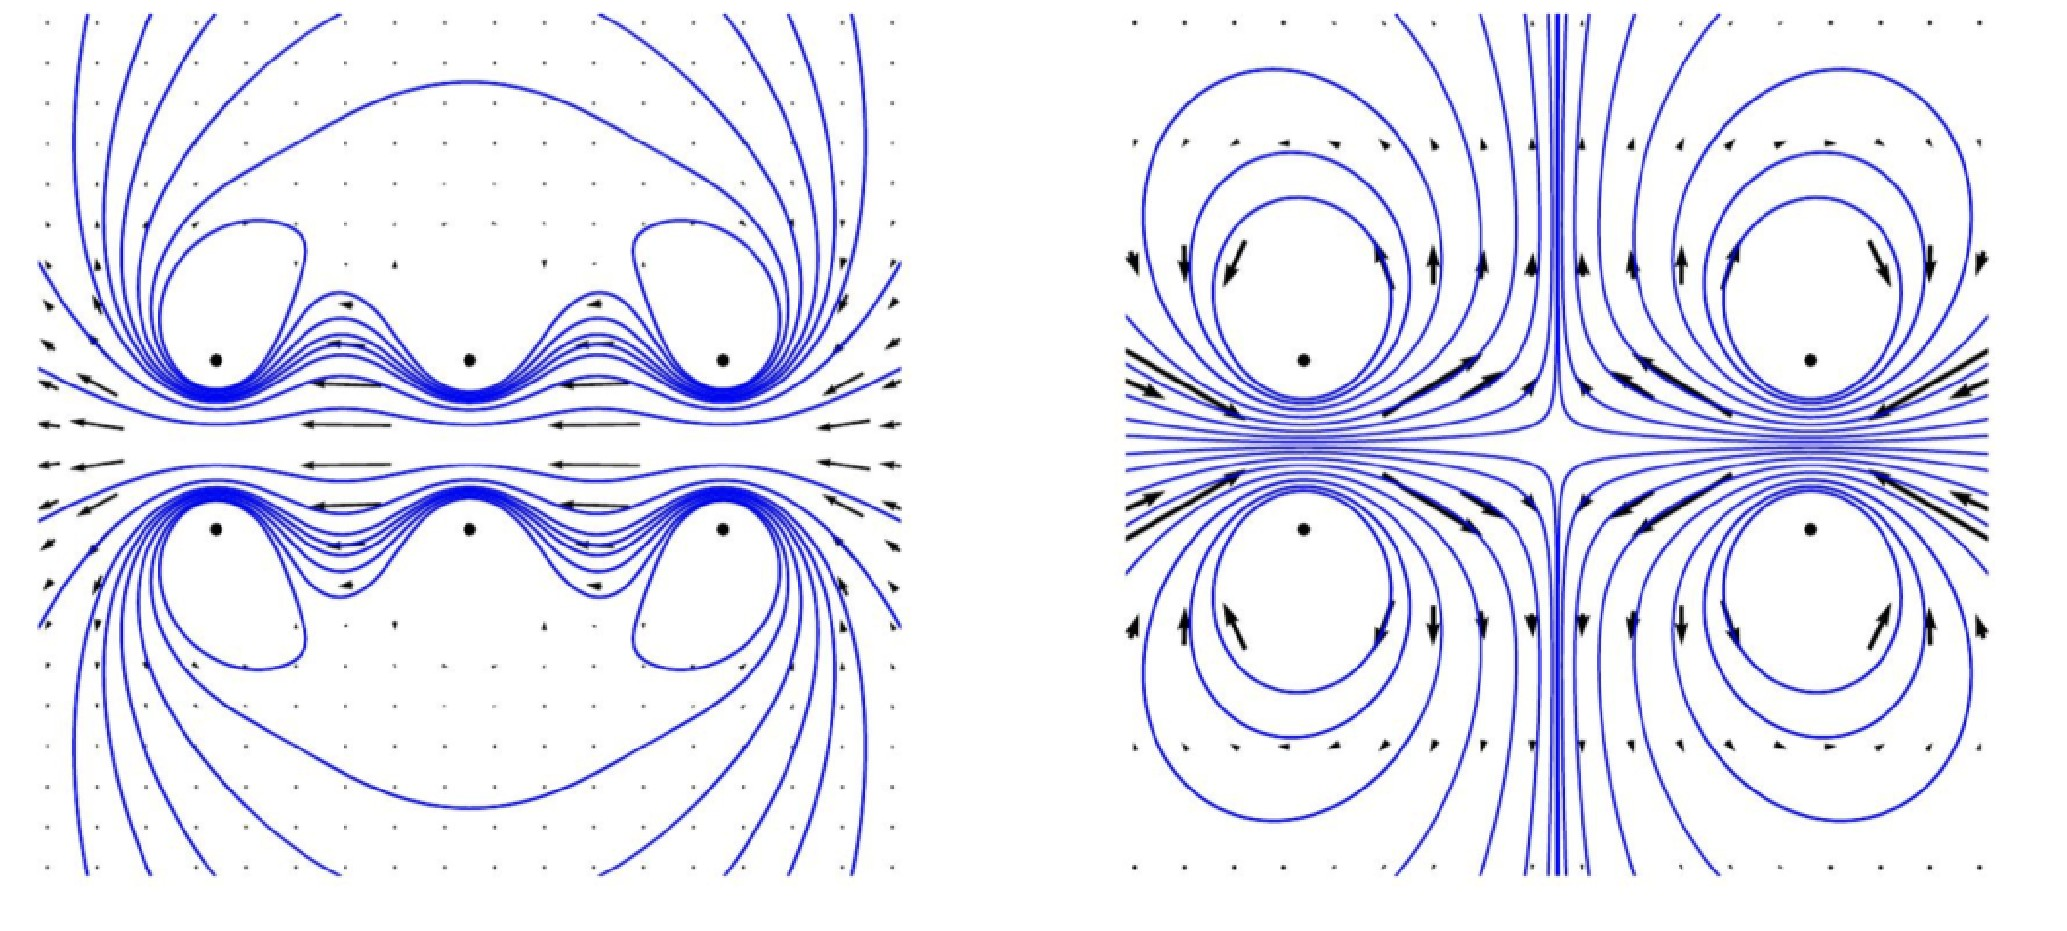
\includegraphics[scale=.5]{../figures/ldc_bilan.jpg}
		\end{center}
	\end{isd}
\end{enumerate}
\noindent
% \begin{tcn}[breakable](appl){Exercice bilan sur lignes de champ}
% 	Les cartes de champ magnétique ci-dessous sont des vues en coupe du champ
% 	produit par des spires de courant circulaires. Dans les deux cas, indiquer
% 	\smallbreak
% 	% \begin{tasks}[label=\protect\fbox{\arabic*}](2)
% 	% 	\task la position des sources
% 	% 	\task le sens du courant circulant dans les spires
% 	% 	\task les zones de champ fort et faible
% 	% 	\task le cas échéant s'il existe une zone de l'espace où le champ magnétique
% 	% 	est uniforme.
% 	% \end{tasks}
% 	\begin{isd}[lefthand ratio=.48]
% 		\begin{enumerate}[label=\sqenumi]
% 			\item la position des sources
% 			\item le sens du courant circulant dans les spires
% 			\item les zones de champ fort et faible
% 			\item le cas échéant s'il existe une zone de l'espace où le champ magnétique
% 			      est uniforme.
% 		\end{enumerate}
% 		\tcblower
% 		\begin{center}
% 			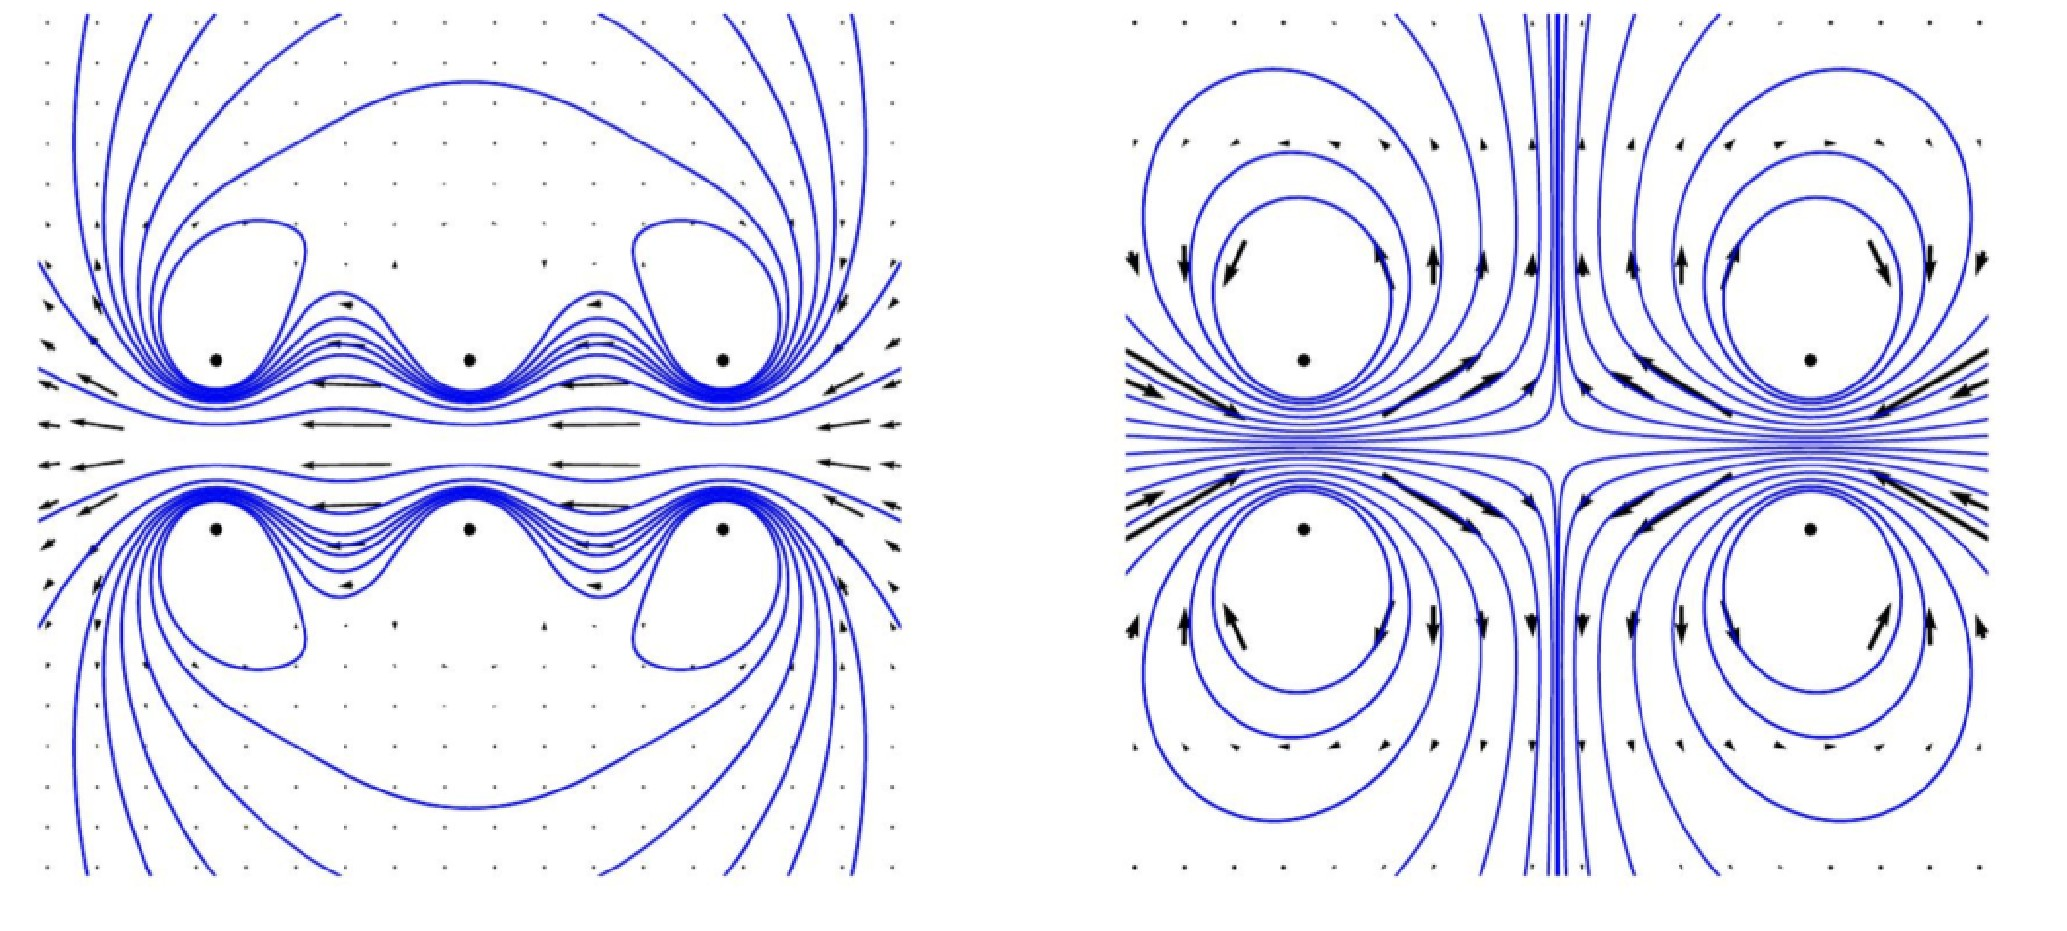
\includegraphics[scale=.5]{../figures/ldc_bilan.jpg}
% 		\end{center}
% 	\end{isd}
% \end{tcn}
\begin{enumerate}[resume, label=\sqenumi]
	\item[s]"3" Présenter les plans de symétrie et d'anti-symétrie d'une
	distribution de courant~: schéma, relations entre $\jf_{\parr}(P)$ et
	$\jf_{\parr}(P')$ d'une part et $\jf_{\perp}(P)$ et $\jf_{\perp}(P')$
	d'autre part. Indiquer alors avec également 2 schémas les propriétés de
	symétrie et d'anti-symétrie du champ magnétique, et ce qu'on retient
	principalement de ces résultats. En utilisant également les propriétés
	d'invariance, déterminer alors les dépendances et la direction de $\Bf
		(M,t)$ d'un fil rectiligne infini.
	\subsection(I2){Actions mécaniques du champ magnétique}
	\item[s]"2" Démontrer les expressions linéique et intégrale de la force de
	\textsc{Laplace} dans une barre conductrice soumise à un champ
	magnétique uniforme et stationnaire. Exprimer alors la puissance de la
	force de \textsc{Laplace}. À l'aide d'un schéma, expliquer l'expérience
	des rails de \textsc{Laplace}.
	\item[s]"3" Établir le couple des actions de \textsc{Laplace} sur une spire
	rectangulaire parcourue par un courant $I$ en rotation autour d'un axe
	de symétrie orthogonal, et plongée dans un champ magnétique extérieur
	uniforme et stationnaire. En déduire la puissance du couple.
	\item[s]"1" À partir de l'expression du couple que subit un aimant dans un
	champ $\Bf$ uniforme et stationnaire, déterminer les positions d'équilibre
	et étudier leur stabilité. Donner alors l'équation régissant le mouvement
	de l'aimant et sa période.
\end{enumerate}

\end{document}
